% vim:encoding=utf8 ft=tex sts=2 sw=2 et:

\documentclass{classrep}
\usepackage[utf8]{inputenc}
\usepackage[a4paper, margin=1in]{geometry}
\usepackage{graphicx}

\studycycle{Matematyka, studia dzienne, mag II st.}
\coursesemester{II}

%\coursename{Angelologia teoretyczna i stosowana}
\coursename{Eksploracja Danych w Javie}
\courseyear{2016/2017}

\courseteacher{dr. Andrzejczak}
\coursegroup{poniedziałek 12:15}

\author{
  \studentinfo{Norbert Landrat}{213518} \and
  \studentinfo{Adrian Grzelak}{213506}
}

\title{Rozpoznawanie podrabianych banknotów}

\begin{document}

\maketitle

\section{Cel projektu}
Projekt polegał na nauce rozpoznawania czy badany banknot jest prawdziwy używając dostępnej bazy danych opisaną w rozdziale 2. Baza zawiera 1372 wpisy z których każdy należy do jednego z 2 rodzajów banknotów (prawdziwy i sfałszowany). Wejściem jest pięć parametrów rzeczywistych, a jako wyjście oczekiwano odpowiedzi, czy badany banknot jest sfałszowany. Przeprowadzono badanie, które miało określić, jaka metoda najlepiej rozwiąże ten problem. Pierwsza metoda użyta do badania dostępnej bazy danych to perceptron wielowarstwowy. Następnie wykorzystano klasyfikator NaiveBayes. Obie metody zostały szczegółowo opisane w dalszych rozdziałach.

\section{Opis danych}
Rozdział ten będzie poświęcony szczegółowemu opisowi danych, które zostaną poddane klasyfikacji. Dane zostały pobrane z repozytorium UCI (https://archive.ics.uci.edu/ml/datasets/banknote+authentication). Autorem powyższych danych jest Volke Lohweg (University of Applied Sciences, Ostwestfalen-Lippe, volker.lohweg '@' hs-owl.de), a donatorem Helene Doerksen (University of Applied Sciences, Ostwestfalen-Lippe, helene.doerksen '@' hs-owl.de). Pochodzą z sierpnia 2012 r.

Dane zostały wydobyte ze zdjęć, które zostały zrobione prawdziwym i sfałszowanym banknotom. W celu transformacji danych na postać cyfrową została użyta kamera przemysłowa, która jest najczęściej używana przy inspekcji wydruku banknotów. Zdjęcia mają wymiary 400 x 400 pikseli. Z powodów technicznych (obiektyw kamery, odległość od badanych przedmiotów) zdjęcia zostały robione w odcieniu szarości  o rozdzielczości 660 dpi. Aby uzyskać konkretne cechy ze zdjęć została użyta transformata falkowa. 

Informacje o atrybutach
\begin{enumerate}
\item wariancja zdjęcia po przekształceniu transformatą falkową
\item skośność zdjęcia po przekształceniu transformatą falkową
\item kurtoza zdjęcia po przekształceniu transformatą falkową
\item entropia zdjęcia
\item klasa
\end{enumerate}
Liczba instancji: 1372

Szczegółowe informacje dotyczące poszczególnych cech
\begin{enumerate}
\item wariancja - wartości numeryczne
\begin{center}
	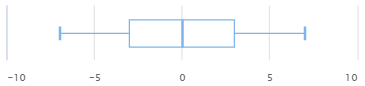
\includegraphics[height=2cm]{wariancja.png}
\end{center}
\item skośność - wartości numeryczne
\begin{center}
	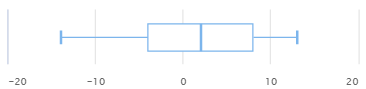
\includegraphics[height=2cm]{skosnosc.png}
\end{center}
\item kurtoza - wartości numeryczne
\begin{center}
	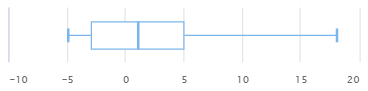
\includegraphics[height=2cm]{kurtoza.png}
\end{center}
\item entropia - wartości numeryczne
\begin{center}
	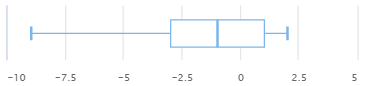
\includegraphics[height=2cm]{entropia.png}
\end{center}
\item klasa – dwie wartości (1 – banknot prawdziwy, 2 – banknot sfałszowany)
\end{enumerate}


\section{Perceptron wielowarstwowy}

Perceptron wielowarstwowy – prosta sieć neuronowa składająca się z co najmniej dwóch neuronów McCullocha-Pittsa ułożonych warstwowo, implementująca algorytm uczenia nadzorowanego klasyfikatorów binarnych. Perceptron wielowarstwowy jest funkcją, która potrafi określić przynależność parametrów wejściowych do jednej z dwóch klas. W przeciwieństwie do perceptronu jednowarstwowego może być wykorzystywany do klasyfikowania zbiorów, które nie są liniowo separowalne.

\begin{center}
	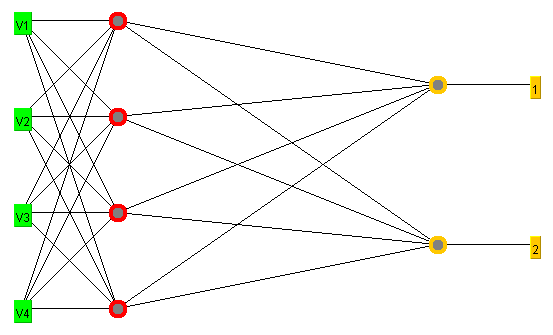
\includegraphics[height=8cm]{siec.png}
	\textbf{Rysunek 1.} Otrzymana sieć neuronowa
\end{center}

Dla celów naszego eksperymentu stowrzyliśmy sieć z 4 neuronami w warstwie ukrytej, przyjęliśmy współczynnik momentum 0.2, Współczynnik nauki 0.3. I ustawiliśmy czas uczenia się zbioru na 1000 epok. Proces uczenia został przeprowadzony metodą kroswalidacji z podziałem na 10 podzbiorów.

Perceptron w tak zdefiniowanym procesie zdołał się nauczyć rozpoznawać elementy ze 100\% skutecznością!

\subsection{Wyniki algorytmu}
\scriptsize
\begin{verbatim}
Podane parametry: -L 0.3 -M 0.2 -N 1000 -V 0 -S 0 -E 20 -H 4 
=====================================================
MultiLayer Perceptron
=====================================================

Correctly Classified Instances        1372              100      %
Incorrectly Classified Instances         0                0      %
Kappa statistic                          1     
Mean absolute error                      0.0022
Root mean squared error                  0.0086
Relative absolute error                  0.4484 %
Root relative squared error              1.7397 %
Total Number of Instances             1372     

=== Confusion Matrix ===

   a   b   <-- classified as
 762   0 |   a = 1
   0 610 |   b = 2
\end{verbatim}
\normalsize


\section{Sieć Bayesowska}
Sieć bayesowska służy do przedstawiania zależności pomiędzy zdarzeniami bazując na rachunku prawdopodobieństwa. Wykorzystuje jeden z ośmiu dostępnych algorytmów szukania. Poniżej przedstawiamy wynik klasyfikacji używając zbioru treningowego oraz 10-krotnej kroswalidacji przy każdym z nich. 
\subsection{Algorytm wyszukiwania K2 (domyślny)}
\subsubsection*{Zbiór treningowy}
\scriptsize 
\begin{verbatim}
==========Sieć Bayesowska z domyślnymi parametrami============

Correctly Classified Instances        1275               92.93   %
Incorrectly Classified Instances        97                7.07   %
Kappa statistic                          0.8559
Mean absolute error                      0.1203
Root mean squared error                  0.2243
Relative absolute error                 24.3602 %
Root relative squared error             45.1457 %
Total Number of Instances             1372     

=== Confusion Matrix ===

   a   b   <-- classified as
 733  29 |   a = 0
  68 542 |   b = 1
\end{verbatim} 
\normalsize
\subsubsection*{10-krotna kroswalidacja}
\scriptsize 
\begin{verbatim}
=== Sieć Bayesowska z domyślnymi parametrami run 1 ===
Classifier: weka.classifiers.bayes.BayesNet -D -Q
weka.classifiers.bayes.net.search.local.K2 -- -P 1 -S BAYES -E
weka.classifiers.bayes.net.estimate.SimpleEstimator -- -A 0.5
Dataset: banknote
Folds: 10
Seed: 1

=== 10-fold Cross-validation run 1===
Correctly Classified Instances        1264               92.1283 %
Incorrectly Classified Instances       108                7.8717 %
Kappa statistic                          0.8399
Mean absolute error                      0.1283
Root mean squared error                  0.2417
Relative absolute error                 25.9856 %
Root relative squared error             48.64   %
Total Number of Instances             1372     
=== Confusion Matrix ===

   a   b   <-- classified as
 722  40 |   a = 0
  68 542 |   b = 1
\end{verbatim} 
\normalsize

\subsection{Algorytm wyszukiwania SimulatedAnnealing}
\subsubsection*{Zbiór treningowy}
\scriptsize 
\begin{verbatim}
==========Sieć Bayesowska z algorytmem szukania:SimulatedAnnealing==========

Correctly Classified Instances        1298               94.6064 %
Incorrectly Classified Instances        74                5.3936 %
Kappa statistic                          0.8904
Mean absolute error                      0.0813
Root mean squared error                  0.1963
Relative absolute error                 16.4604 %
Root relative squared error             39.5127 %
Total Number of Instances             1372     

=== Confusion Matrix ===

   a   b   <-- classified as
 735  27 |   a = 0
  47 563 |   b = 1
\end{verbatim} 
\normalsize
\subsubsection*{10-krotna kroswalidacja}
\scriptsize 
\begin{verbatim}
=== Sieć Bayesowska z algorytmem szukania:SimulatedAnnealing run 1 ===
Classifier: weka.classifiers.bayes.BayesNet -D -Q
weka.classifiers.bayes.net.search.global.SimulatedAnnealing -- -A 10.0 -U
10000 -D 0.999 -R 1 -S LOO-CV -E weka.classifiers.bayes.net.estimate.SimpleEstimator -- -A 0.5
Dataset: banknote
Folds: 10
Seed: 1

=== 10-fold Cross-validation run 1===
Correctly Classified Instances        1321               96.2828 %
Incorrectly Classified Instances        51                3.7172 %
Kappa statistic                          0.9246
Mean absolute error                      0.064 
Root mean squared error                  0.169 
Relative absolute error                 12.9677 %
Root relative squared error             34.0047 %
Total Number of Instances             1372     
=== Confusion Matrix ===

   a   b   <-- classified as
 743  19 |   a = 0
  32 578 |   b = 1
\end{verbatim} 
\normalsize

\subsection{Algorytm wyszukiwania TabuSearch}
\subsubsection*{Zbiór treningowy}
\scriptsize 
\begin{verbatim}
============Sieć Bayesowska z algorytmem szukania:TabuSearch==========

Correctly Classified Instances        1275               92.93   %
Incorrectly Classified Instances        97                7.07   %
Kappa statistic                          0.8559
Mean absolute error                      0.1203
Root mean squared error                  0.2243
Relative absolute error                 24.3602 %
Root relative squared error             45.1457 %
Total Number of Instances             1372     

=== Confusion Matrix ===

   a   b   <-- classified as
 733  29 |   a = 0
  68 542 |   b = 1
\end{verbatim} 
\normalsize
\subsubsection*{10-krotna kroswalidacja}
\scriptsize 
\begin{verbatim}
=== Sieć Bayesowska z algorytmem szukania:TabuSearch run 1 ===
Classifier: weka.classifiers.bayes.BayesNet -D -Q
weka.classifiers.bayes.net.search.global.TabuSearch -- -L 5 -U 10 -P 1 -S
LOO-CV -E weka.classifiers.bayes.net.estimate.SimpleEstimator -- -A 0.5
Dataset: banknote
Folds: 10
Seed: 1

=== 10-fold Cross-validation run 1===
Correctly Classified Instances        1264               92.1283 %
Incorrectly Classified Instances       108                7.8717 %
Kappa statistic                          0.8399
Mean absolute error                      0.1283
Root mean squared error                  0.2417
Relative absolute error                 25.9856 %
Root relative squared error             48.64   %
Total Number of Instances             1372     
=== Confusion Matrix ===

   a   b   <-- classified as
 722  40 |   a = 0
  68 542 |   b = 1
\end{verbatim} 
\normalsize

\subsection{Algorytm wyszukiwania TAN}
\subsubsection*{Zbiór treningowy}
\scriptsize 
\begin{verbatim}
==========Sieć Bayesowska z algorytmem szukania:TAN==========

Correctly Classified Instances        1298               94.6064 %
Incorrectly Classified Instances        74                5.3936 %
Kappa statistic                          0.8904
Mean absolute error                      0.0833
Root mean squared error                  0.1966
Relative absolute error                 16.8604 %
Root relative squared error             39.5613 %
Total Number of Instances             1372     

=== Confusion Matrix ===

   a   b   <-- classified as
 735  27 |   a = 0
  47 563 |   b = 1
\end{verbatim} 
\normalsize
\subsubsection*{10-krotna kroswalidacja}
\scriptsize 
\begin{verbatim}
=== Sieć Bayesowska z algorytmem szukania:TAN run 1 ===
Classifier: weka.classifiers.bayes.BayesNet -D -Q
weka.classifiers.bayes.net.search.global.TAN -- -S LOO-CV -E
weka.classifiers.bayes.net.estimate.SimpleEstimator -- -A 0.5
Dataset: banknote
Folds: 10
Seed: 1

=== 10-fold Cross-validation run 1===
Correctly Classified Instances        1310               95.481  %
Incorrectly Classified Instances        62                4.519  %
Kappa statistic                          0.9082
Mean absolute error                      0.0772
Root mean squared error                  0.1828
Relative absolute error                 15.6265 %
Root relative squared error             36.7806 %
Total Number of Instances             1372     
=== Confusion Matrix ===

   a   b   <-- classified as
 741  21 |   a = 0
  41 569 |   b = 1
\end{verbatim} 
\normalsize

\subsection{Algorytm wyszukiwania GeneticSearch}
\subsubsection*{Zbiór treningowy}
\scriptsize 
\begin{verbatim}
==========Sieć Bayesowska z algorytmem szukania:GeneticSearch==========

Correctly Classified Instances        1298               94.6064 %
Incorrectly Classified Instances        74                5.3936 %
Kappa statistic                          0.8904
Mean absolute error                      0.0788
Root mean squared error                  0.1963
Relative absolute error                 15.9485 %
Root relative squared error             39.5109 %
Total Number of Instances             1372     

=== Confusion Matrix ===

   a   b   <-- classified as
 735  27 |   a = 0
  47 563 |   b = 1
\end{verbatim} 
\normalsize
\subsubsection*{10-krotna kroswalidacja}
\scriptsize 
\begin{verbatim}
=== Sieć Bayesowska z algorytmem szukania:GeneticSearch run 1 ===
Classifier: weka.classifiers.bayes.BayesNet -D -Q
weka.classifiers.bayes.net.search.global.GeneticSearch -- -L 10 -A 100 -U
10 -R 1 -M -C -S LOO-CV -E weka.classifiers.bayes.net.estimate.SimpleEstimator -- -A 0.5
Dataset: banknote
Folds: 10
Seed: 1

=== 10-fold Cross-validation run 1===
Correctly Classified Instances        1319               96.137  %
Incorrectly Classified Instances        53                3.863  %
Kappa statistic                          0.9216
Mean absolute error                      0.0586
Root mean squared error                  0.1706
Relative absolute error                 11.8624 %
Root relative squared error             34.3286 %
Total Number of Instances             1372     
=== Confusion Matrix ===

   a   b   <-- classified as
 741  21 |   a = 0
  32 578 |   b = 1
\end{verbatim} 
\normalsize

\subsection{Algorytm wyszukiwania HillClimber}
\subsubsection*{Zbiór treningowy}
\scriptsize 
\begin{verbatim}
==========Sieć Bayesowska z algorytmem szukania:HillClimber==========

Correctly Classified Instances        1275               92.93   %
Incorrectly Classified Instances        97                7.07   %
Kappa statistic                          0.8559
Mean absolute error                      0.1203
Root mean squared error                  0.2243
Relative absolute error                 24.3602 %
Root relative squared error             45.1457 %
Total Number of Instances             1372     

=== Confusion Matrix ===

   a   b   <-- classified as
 733  29 |   a = 0
  68 542 |   b = 1
\end{verbatim} 
\normalsize
\subsubsection*{10-krotna kroswalidacja}
\scriptsize 
\begin{verbatim}
=== Sieć Bayesowska z algorytmem szukania:HillClimber run 1 ===
Classifier: weka.classifiers.bayes.BayesNet -D -Q
weka.classifiers.bayes.net.search.global.HillClimber -- -P 1 -S LOO-CV -E
weka.classifiers.bayes.net.estimate.SimpleEstimator -- -A 0.5
Dataset: banknote
Folds: 10
Seed: 1

=== 10-fold Cross-validation run 1===
Correctly Classified Instances        1264               92.1283 %
Incorrectly Classified Instances       108                7.8717 %
Kappa statistic                          0.8399
Mean absolute error                      0.1283
Root mean squared error                  0.2417
Relative absolute error                 25.9856 %
Root relative squared error             48.64   %
Total Number of Instances             1372     
=== Confusion Matrix ===

   a   b   <-- classified as
 722  40 |   a = 0
  68 542 |   b = 1
\end{verbatim} 
\normalsize

\subsection{Algorytm wyszukiwania LAGDHillClimber}
\subsubsection*{Zbiór treningowy}
\scriptsize 
\begin{verbatim}
==========Sieć Bayesowska z algorytmem szukania:LAGDHillClimber==========

Correctly Classified Instances        1248               90.9621 %
Incorrectly Classified Instances       124                9.0379 %
Kappa statistic                          0.815 
Mean absolute error                      0.1275
Root mean squared error                  0.2371
Relative absolute error                 25.8185 %
Root relative squared error             47.7104 %
Total Number of Instances             1372     

=== Confusion Matrix ===

   a   b   <-- classified as
 733  29 |   a = 0
  95 515 |   b = 1
\end{verbatim} 
\normalsize
\subsubsection*{10-krotna kroswalidacja}
\scriptsize 
\begin{verbatim}
=== Sieć Bayesowska z algorytmem szukania:LAGDHillClimber run 1 ===
Classifier: weka.classifiers.bayes.BayesNet -D -Q
weka.classifiers.bayes.net.search.local.LAGDHillClimber -- -L 2 -G 5 -P 1
-S BAYES -E weka.classifiers.bayes.net.estimate.SimpleEstimator -- -A 0.5
Dataset: banknote
Folds: 10
Seed: 1

=== 10-fold Cross-validation run 1===
Correctly Classified Instances        1245               90.7434 %
Incorrectly Classified Instances       127                9.2566 %
Kappa statistic                          0.811 
Mean absolute error                      0.1344
Root mean squared error                  0.249 
Relative absolute error                 27.2083 %
Root relative squared error             50.1161 %
Total Number of Instances             1372     
=== Confusion Matrix ===

   a   b   <-- classified as
 724  38 |   a = 0
  89 521 |   b = 1
\end{verbatim} 
\normalsize

\subsection{Algorytm wyszukiwania RepeatedHillClimber}
\subsubsection*{Zbiór treningowy}
\scriptsize 
\begin{verbatim}
==========Sieć Bayesowska z algorytmem szukania:RepeatedHillClimber==========

Correctly Classified Instances        1275               92.93   %
Incorrectly Classified Instances        97                7.07   %
Kappa statistic                          0.8559
Mean absolute error                      0.1203
Root mean squared error                  0.2243
Relative absolute error                 24.3602 %
Root relative squared error             45.1457 %
Total Number of Instances             1372     

=== Confusion Matrix ===

   a   b   <-- classified as
 733  29 |   a = 0
  68 542 |   b = 1
\end{verbatim} 
\normalsize
\subsubsection*{10-krotna kroswalidacja}
\scriptsize 
\begin{verbatim}
=== Sieć Bayesowska z algorytmem szukania:RepeatedHillClimber run 1 ===
Classifier: weka.classifiers.bayes.BayesNet -D -Q
weka.classifiers.bayes.net.search.global.RepeatedHillClimber -- -U 10 -A 1
-P 1 -S LOO-CV -E weka.classifiers.bayes.net.estimate.SimpleEstimator -- -A 0.5
Dataset: banknote
Folds: 10
Seed: 1

=== 10-fold Cross-validation run 1===
Correctly Classified Instances        1264               92.1283 %
Incorrectly Classified Instances       108                7.8717 %
Kappa statistic                          0.8399
Mean absolute error                      0.1283
Root mean squared error                  0.2417
Relative absolute error                 25.9856 %
Root relative squared error             48.64   %
Total Number of Instances             1372     
=== Confusion Matrix ===

   a   b   <-- classified as
 722  40 |   a = 0
  68 542 |   b = 1
\end{verbatim} 
\normalsize

\subsection{Podsumowanie i wnioski}
\begin{tabular}{|l|r|r|}
  \hline 
  Algorytm szukania & Zbiór Treningowy & 10-krotna walidacj \\
  \hline
  K2 & 92,93\% & 92,1283\% \\
  \hline
  SimulatedAnnealing & 94,6064\% & 96,2828\% \\
  \hline
  TabuSearch & 92,93\% & 92,1283\% \\
  \hline
  TAN & 94,6064\% & 95,481\% \\
  \hline
  GeneticSearch & 94,6064\% & 96,137\% \\ 
  \hline
  HillClimber & 92,93\% & 92,1283\% \\
  \hline
  LAGDHillClimber & 90,9621\% & 90,7434\% \\
  \hline
  RepeatedHillClimber & 92,93\% & 92,1283\% \\
  \hline
\end{tabular} \smallskip

Najwyższą skuteczność uzyskuje algorytm wyszukiwania SimulatedAnnealing, jednakże okraszone jest to wysokim czasem obliczeniowym. W przypadku większej liczby danych algorytm mógłby się okazać wysoce nieefektywny. Niewiele mniej skutecznym pozostają algorytmy TAN i GeneticSearch o szybszym działaniu i skuteczności przy 10-krotnej kroswalidacji kolejno: 95,481\%; 96,137\%.

 

\section{Istotność atrybutów}

Istotność atrybutów badamy na 3 sposoby
\subsection{Miara Relief}
Miara Relief to wynik działania algorytmu wyznaczającego relatywną ważność atrybutów. Ocenia jak dobrze poszczególne atrybuty nadają się do przewidywania wartości jednego wybranego atrybutu binarnego, tzw. atrybutu decyzyjnego. Poniżej zaprezentowany został ranking istotności atrybutów przy użyciu domyślnych parametrów, tzn. Attribute Evaluator – ReliefFAttributeEval o liczbie sąsiadów – 10, Search Method – Ranker. 

\scriptsize
\begin{verbatim}
=== Run information ===

Evaluator:    weka.attributeSelection.ReliefFAttributeEval -M -1 -D 1 -K 10
Search:       weka.attributeSelection.Ranker -T -1.7976931348623157E308 -N -1
Relation:     banknote-authentication
Instances:    1372
Attributes:   5
              Variance
              Skewness
              Curtosis
              Entropy
              Class
Evaluation mode:    evaluate on all training data



=== Attribute Selection on all input data ===

Search Method:
	Attribute ranking.

Attribute Evaluator (supervised, Class (nominal): 5 Class):
	ReliefF Ranking Filter
	Instances sampled: all
	Number of nearest neighbours (k): 10
	Equal influence nearest neighbours

Ranked attributes:
 0.1272  1 Variance
 0.1006  2 Skewness
 0.0647  3 Curtosis
 0.0213  4 Entropy

Selected attributes: 1,2,3,4 : 4

\end{verbatim}
\normalsize

Badanie wykazuje że decyzja jest najbardziej uzależniona od wariancji, oraz w niewiele mniejszym stopniu od skośności. Kurtoza odgrywa mniejszą rolę przy podejmowaniu decyzji, natomiast entropia ma już znikomy wpływ.

\subsection{Analiza histogramów}

Rozkład zmiennych decyzyjnych w naszych danych prezentuje się następująco:
\begin{center}
	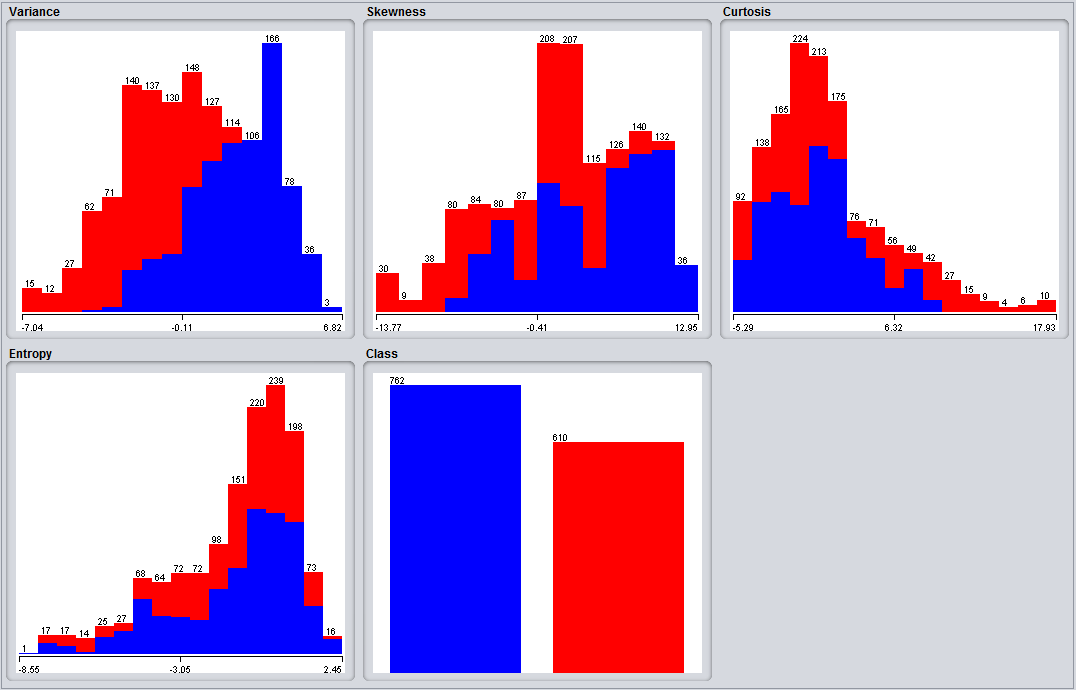
\includegraphics[height=10cm]{rozklad_parametrow.png}
	\textbf{Rysunek 1.} Histogramy dla poszczególnych parametrów
\end{center}

Jeżeli spojrzymy na wykresy wariancji ewidentnie potwierdza nam się założenie że jest istotnie najbardziej skorelowana z podjętą decyzją. Widać że elementy dla poszczególnych decyzji są zupełnie inaczej rozłożone. Zupełnie inaczej sytuacja ma się w przypadku Entropii. Tam rozłożenie jednych i drugich wygląda niemal identycznie.

\subsection{Analiza wag w neuronach perceptronu}
W wyniku działania algorytmu multilayerPerceptron otrzymaliśmy pewne wagi na poszczególnych neuronach w sieci:

\scriptsize
\begin{verbatim}
Sigmoid Node 0
    Inputs    Weights
    Threshold    -15.70582061524466
    Node 2    2.5380086425502792
    Node 3    12.55495230795682
    Node 4    9.472054016485565
    Node 5    9.578991234475602
Sigmoid Node 1
    Inputs    Weights
    Threshold    15.704150716426224
    Node 2    -2.5072841574455755
    Node 3    -12.552365481893666
    Node 4    -9.47523047158287
    Node 5    -9.581266354029816
Sigmoid Node 2
    Inputs    Weights
    Threshold    -0.23529049334696428
    Attrib Variance    4.772455188120188
    Attrib Skewness    1.6873893615432696
    Attrib Curtosis    3.7592737494056543
    Attrib Entropy    -0.29719915903371485
Sigmoid Node 3
    Inputs    Weights
    Threshold    2.7664652585933185
    Attrib Variance    7.3696398807362336
    Attrib Skewness    13.591522498703414
    Attrib Curtosis    11.980966729289058
    Attrib Entropy    1.053349663764041
Sigmoid Node 4
    Inputs    Weights
    Threshold    5.9345495765525165
    Attrib Variance    4.537498776242926
    Attrib Skewness    -0.8813154253219377
    Attrib Curtosis    10.67428507310192
    Attrib Entropy    -1.2575630002344076
Sigmoid Node 5
    Inputs    Weights
    Threshold    5.819967131416015
    Attrib Variance    12.507385423812616
    Attrib Skewness    7.338449459299226
    Attrib Curtosis    5.644381683569787
    Attrib Entropy    -5.1252118033263905
\end{verbatim}
\normalsize

Dają one nam również pewien pogląd na to jak bardzo wybór jest uzależniony od poszczególnych parametrów (Widzimy że mnożniki przy Entropii są niskie W porównaniu do tych które obserwujemy przy Wariancji)

\section{Wnioski z badania}
Analizowany zbiór jest bardzo trafnie dobrany do celów klasyfikowania. Dane w przypadku metody perceptronu wielowarstwowego są klasyfikowane z wysoką skutecznością (dochodząc do 100\%), co może oznaczać, że metoda sprawdzania sfałszowanych banknotów może znaleźć odzwierciedlenie w rzeczywistości. W procesie nauczania perceptronu duży wpływ na osiągane wyniki ma ilość neuronów w wartswie ukrytej. Zbyt mała ich ilość może doprowadzić do słabego nauczenia się wzorca, natomiast zbyt duża do zjawiska przeuczenia (Perceptron doskonale rozpoznaje elementy ze zbioru nauczającego, ale natrafia na problemy przy danych pochodzących spoza tego zbioru. Klasyfikator Naiwny Bayes nie poradził sobie z tym zadaniem równie dobrze - klasyfikacja ze sktucznością około 95\% w przypadku systemów sprawdzających autentyczność banknotów pomimo tego że brzmi imponująco, może prowadzić do znacznych strat finansowych.

\end{document}
